\linespread{1.5}
%use \usepackage{float}
\textbf{Solução}

\textbf{a)}
\begin{figure}[H]
    \centering
    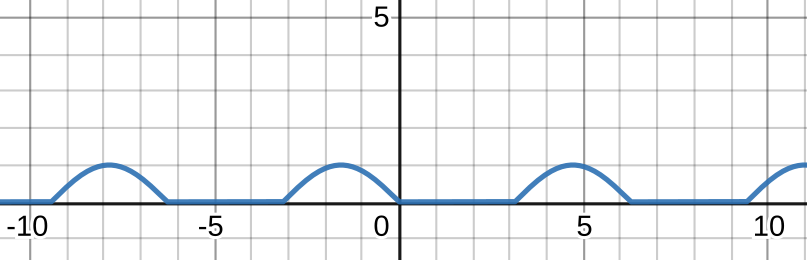
\includegraphics[width = 0.7\linewidth]{fig/sf9.png}
    \caption{Feita pelo site \textit{https://www.desmos.com/calculator}.}
\end{figure}
\textbf{b)}
Dada a série de Fourier complexa:
\begin{equation}
    \label{eq:Fouriercomplexa}
    f(x) = \sum^{+\infty}_{k=-\infty} c_k e^{ikwx}
\end{equation}
onde, 
\begin{equation}
    \label{eq:ckFouerier}
    c_k = \frac{1}{T} \int^T_0 f(x)e^{-ikwx}dx
\end{equation}

Neste caso também temos que $T=2\pi$ e portanto $w = 1$.

\begin{equation*}
    c_k = \frac{1}{2\pi}\left(\int_{-\pi}^0 0e^{-ikx}dx + \int^\pi_0 \sin{(x)}e^{-ikx}dx\right) = \frac{1}{2\pi}\int^\pi_0 \sin{(x)}e^{-ikx}dx = \frac{1}{2\pi}(I)
\end{equation*}
\begin{equation*}
    (I) =  \int^\pi_0 \sin{(x)}e^{-ikx}dx = \left[\frac{\sin{(x)}e^{-ikx}}{-ik}\right]^\pi_0 - \int^\pi_0 \frac{\cos{(x)}e^{-ikx}}{-ik}dx\
\end{equation*}
\begin{equation*}
    \int^\pi_0 \sin{(x)}e^{-ikx}dx = \left[\frac{\sin{(x)}e^{-ikx}}{-ik}\right]^\pi_0 + \left[\frac{cos(x)e^{-ikx}}{-(ik)^2}\right]^\pi_0 - \int^\pi_0 \frac{\sin{(x)}e^{-ikx}dx}{(ik)^2}
\end{equation*}
isolando os termos que contem a equação $(I)$:
\begin{equation*}
    \left[1+\frac{1}{(ik)^2}\right]\int^\pi_0 \sin{(x)}e^{-ikx}dx = \left[\frac{\sin{(x)}e^{-ikx}}{-ik}\right]^\pi_0 + \left[\frac{cos(x)e^{-ikx}}{-(ik)^2}\right]^\pi_0
\end{equation*}
sabemos que $sin(\pi) = sin(0) = 0$, logo simplificamos:
\begin{equation*}
    (I) = \frac{(ik)^2}{1+(ik)^2}\frac{1}{(ik)^2}\left[-cos(x)e^{-ikx}\right]^\pi_0 = \frac{1}{1+(ik)^2}(-cos(\pi)e^{-ik\pi} + cos(0)e^0) = \frac{1}{1+(ik)^2}(1 - e^{-ik\pi}) 
\end{equation*}
\begin{equation*}
    (I) = \frac{1}{1 - k^2}[1 - (cos(k\pi) + i\sin(k\pi))] = \frac{1-(-1)^k}{1-k^2}
\end{equation*}
Dessa forma podemos afirmar que, neste caso:
\begin{equation}
    c_k = \frac{1}{2\pi}\frac{1-(-1)^k}{1-k^2} 
\end{equation}
Note que para todo $k$ par, $c_k=0$, o que não ocorre para $k$ ímpar. Dessa forma:
\begin{equation}
    \label{eq:sf9ck}
    c_{2k-1} = \frac{1}{2\pi}\frac{1-(-1)^{2k-1}}{1-(2k-1)^2}
\end{equation}

Subistituindo então \ref{eq:sf9ck} em \ref{eq:Fouriercomplexa}, obtemos que:
\begin{equation}
    \boxed{f(x) = \sum^\infty_{-\infty} \frac{1}{2\pi}\frac{1-(-1)^{2k-1}}{1-(2k-1)^2}e^{kx} }
\end{equation}
\underline{Para todo $k\in\Z$ exceto $k=0$, ou $k=1$.}